\chapter{研究内容}
\label{cha:content}

\section{问题的数学模型}\label{section:model}

\subsection[非协作定位场景]{非协作定位场景}\label{subsection:noncooperative_localization}

{单个节点定位}

        考虑一个平面定位场景中部署了$N_b$个位置已知的\textcolor{blue}{锚点},锚点的位置记为$\{\bm{p}^b_1,\bm{p}^b_2,...\bm{p}^b_{N_b}\}$,现在要对场景中一个\textcolor{blue}{位置未知}的节点进行定位,待定位节点的位置为$\bm{p}$,如图(\ref{fig:non_cooperative_spatial})所示。
        \begin{figure}
          \centering
          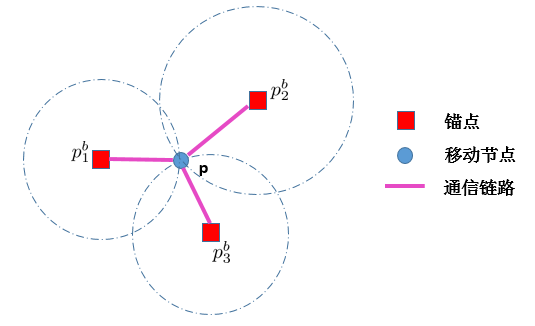
\includegraphics[width=300pt]{non_cooperative_spatial.png}
          \caption{非协作静态场景下的定位}\label{fig:non_cooperative_spatial}
        \end{figure}
假设\textcolor{blue}{待定位节点}和每一个锚点都可以相互通信进行无线测距,距离测量量服从均值为$||\bm{p}^b_i-\bm{p}||$,方差为$\sigma_i$的正态分布$X_i$。

$N_b$个\textcolor{blue}{独立}测量量的联合概率分布为:
\begin{equation}\label{eq:single}
f(x_1,...x_{N_b}|\textbf{p})=\prod_{i=1}^{N_b}\frac{1}{\sqrt{2\pi\sigma_i^2}}exp(-\frac{(x_i-||\bm{p}^b_i-\bm{p}||)^2}{2\sigma_i^2})
\end{equation}

根据点估计的理论,对于一个无偏估计量,它的方差的下界是\textcolor{blue}{费舍尔信息量}(Fisher Information)的倒数,称之为\textcolor{blue}{克拉美罗界}(Crame Rao Bound),在本文的讨论中,也称之为定位误差下界(Spatial Position Error Bound),它的计算公式为:
\begin{equation}\label{eq:SPEB_formula}
  \text{SPEB}=\text{tr}(\bm{I(\bm{p})}^{-1})
\end{equation}
  % - A title should summarize the slide in an understandable fashion
  %   for anyone how does not follow everything on the slide itself.


{费舍尔信息矩阵}
以节点的\textcolor{blue}{2维}位置为待估计参数,费舍尔信息量推广为\textcolor{blue}{费舍尔信息矩阵}(Fisher Information Matrix)。

对于我们的模型问题,费舍尔信息矩阵有如下的形式:
\begin{equation}\label{eq:uu}
I(\bm{p})=\displaystyle\sum_{i=1}^{N_b}\frac{1}{\sigma_i^2}\bm{u}_i\bm{u}_i^T
\end{equation}
其中
\begin{equation}
\bm{u_i}=\frac{\bm{p}^b_i-\bm{p}}{||\bm{p}^b_i-\bm{p}||}
\end{equation}


\subsection[协作定位场景]{协作定位场景}\label{subsection:cooperative_localization}

多个待测节点协作定位

考虑一个平面定位场景中不仅部署了$N_b$个位置已知的锚点,还有$N_a$个位置未知的待定位节点,某些位置未知的节点之间可以\textcolor{blue}{彼此测距},如图(\ref{fig:cooperative_spatial})所示。第i和第j个未知节点距离测量量服从均值为$||\bm{p}^a_i-\bm{p}^a_j||)$,方差为$\sigma_{ij}$的正态分布$X_{ij}$。
        \begin{figure}
          \centering
          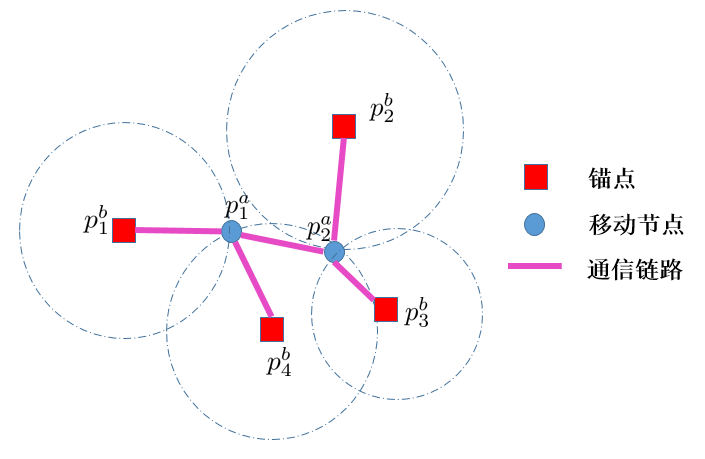
\includegraphics[width=300pt]{cooperative_spatial.png}
          \caption{协作静态场景下的定位}\label{fig:cooperative_spatial}
        \end{figure}

以$N_a$个未知节点的位置$\{p_i\}$作为待估计的参数,可以得到测距量的联合概率密度函数为

\begin{equation}
\prod_{i=1}^{N_a} f(x^i_1,...x^{i}_{N_b}|\bm{p_i})\prod_{(i,j)\in \mathcal{E}}\frac{1}{\sqrt{2\pi\sigma_{ij}^2}}exp(-\frac{(x_{ij}-||\bm{p}_i-\bm{p}_j||)^2}{2\sigma_{ij}^2})
\end{equation}
上式中f的具体表达式为式(\ref{eq:single}),$\mathcal{E}$表示可以彼此测距的未知节点的二元组的集合,而$x_t^i$表示第t个锚点和第i个未知节点的距离测量量。

\textbf{费舍尔信息矩阵}

仿照单节点时费舍尔信息矩阵的推导,关于$2N_a$个参数$\{p_i^a\}$的费舍尔信息矩阵$I(\bm{p}_1,\dots,\bm{p}_{N_a})$有如下的表达形式:
\begin{equation}
\scriptsize{
I(\bm{p}_1,\dots,\bm{p}_{N_a})=
\left(
\begin{array}{cccc}
I(\bm{p}_1)+&-\bm{C}_{1,2}&...&-\bm{C}_{1,N_a}\\
\sum_{j\in \{1,..N_a\}\backslash\{1\}}\bm{C}_{1,j}&&&\\
&&&\\
-\bm{C}_{1,2} & I(\bm{p}_2)+
&...&-\bm{C}_{2,N_a}\\
&\sum_{j\in \{1,..N_a\}\backslash \{2\}}\bm{C}_{2,j}&&\\
&&&\\
\vdots &\vdots&\ddots &\vdots\\
&&&\\
&&&I(\bm{p}_{N_a})+\\
-\bm{C}_{1,N_a}&-\bm{C}_{2,N_a}&...& \sum_{j\in \{1,..N_a\}\backslash\{N_a\}}\bm{C}_{N_a,j}\\
\end{array}
\right)
}
\end{equation}
上面的式子中$I(\bm{p}_i)$表示$N_b$个锚点对未知节点距离测量的贡献,和前面的(\ref{eq:uu})式相同。$C_{i,j}=\bm{1}_{(i,j)\in E}\bm{u}_{ij}\bm{u}_{ij}^T/\sigma^2_{ij}$,表示未知节点i和j协作的矩阵。
$\bm{u}_{ij}=\frac{\bm{p}_i-\bm{p}_j}{||\bm{p}_i-\bm{p}_j||}$表示未知节点i和j的方向向量。
\subsection[时间协作定位]{时间协作定位}\label{subsection:temporal_cooperative_localization}

\textbf{单个待测节点时间协作定位}
考虑一个平面定位场景中有一个待定位的移动节点,场景中部署的$N_b$个位置已知的锚点分别在在$t_1,\dots,t_{N_a}$时刻对该节点进行定位,移动节点可以通过自身的加速度传感器对自己的速度有测量,如图(\ref{fig:cooperative_single_temporal})所示。
        \begin{figure}
          \centering
          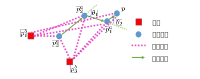
\includegraphics[width=300pt]{cooperative_single_temporal.png}
          \caption{协作动态场景下的定位}\label{fig:cooperative_single_temporal}
        \end{figure}

假设测量时间间隔比较小使得相邻测量间节点速度方向可近似看作不变,速度测量值服从均值为$v$,方差为$\sigma_{v}$的正态分布$V_{ij}$。
那么以节点各时刻的的位置$\{p_i\}$作为待估计的参数,可以得到包括相邻时刻间的所有测距量的联合概率密度函数为
\begin{equation}
\prod_{i=1}^{N_a} f(x^i_1,...x^{i}_{N_b}|\bm{p_i})
\prod_{i=1}^{N_a-1}\frac{1}{\sqrt{2\pi}\sigma_v(t_{i+1}-t_i)}
exp(-\frac{(v_{i,i+1}(t_{i+1}-t_i)-||\bm{p}_i-\bm{p}_{i+1}||)^2}{2\sigma_v^2(t_{i+1}-t_i)^2})
\end{equation}
{费舍尔信息矩阵}
关于$2N_a$个参数$\{p_i\}$的费舍尔信息矩阵有如下的表达形式:
\begin{equation}\label{eq:time_cooperation_matrix}
\scriptsize{
I(\bm{p}_1,\dots,\bm{p}_{N_a})=
\left(
\begin{array}{ccccc}
I(\bm{p}_1)+\bm{C}_{1,2}&-\bm{C}_{1,2}&\bm{0}&\dots&\bm{0}\\
&&&&\\
-\bm{C}_{1,2} & I(\bm{p}_2)+\bm{C}_{1,2}+\bm{C}_{2,3}&-\bm{C}_{2,3}&\dots&\bm{0}\\
\vdots &\vdots&\ddots &\vdots&\vdots\\
&&&&\\
\bm{0}&\bm{0}&...& -\bm{C}_{N_a-1,N_a}&\bm{C}_{N_a-1,N_a}+I(\bm{p}_{N_a})\\
\end{array}
\right)
}
\end{equation}
上面的式子中若将2乘2的矩阵看作单位元素,则是一个三对角的矩阵。$I(\bm{p}_i)$表示$N_b$个锚点对未知节点距离测量的贡献,和前面的(\ref{eq:uu})式相同。$C_{i,i+1}=\bm{1}_{(i,j)\in E}\bm{u}_{ij}\bm{u}_{ij}^T/(\sigma_v^2(t_{i+1}-t_i)^2)$,表示未知节点i和j协作的矩阵,$\bm{u}_{ij}$表示未知节点i和j的方向向量。

我们可以将第二个模型问题与线性网络单节点时间协作建立联系,只需对上面概率密度函数中出现的符号重排即可:
将两移动节点在$t_1$时刻的协作的边作为链路的中心,该链路记为$l$,左右各有$N_a$个节点,分别表示各节点$t_i$时刻的位置。
以其中一个移动节点为参照,研究其$t_{N_a}$时刻的位置在有无$l$的影响,无$l$时,协作链路长度只有$N_a-1$,有$l$时,协作链路长度是$2N_a-1$,增加了$N_a$条链路的协作信息。于是得到的费舍尔信息矩阵与式(\ref{eq:time_cooperation_matrix})形式相同,维数为$4N_a$。

\textbf{两个节点时间协作定位}
考虑一个平面定位场景中有两个待定位的移动节点$p,q$,在初始时刻$t_1$两个移动节点之间有一次测距,服从无偏的标准差为$\sigma$的正态分布,之后时刻$t_2,\dots,t_{N_a}$两个节点不再协作,在各个时刻场景中部署的$N_b$个位置已知的锚点都可以对两个节点进行定位,移动节点可以通过自身的加速度传感器对自己的速度有测量,
假设时间间隔比较小使得相邻测量间节点速度方向可近似看作不变,速度测量值分别服从方差为$\sigma_i$的正态分布$V_i$和标准差为$\sigma'_j$的正态分布$V'_i$(均值未知,但测量是无偏的),同时假设每个节点从$t_i$到$t_{i+1}$时刻的角度符从$[0,2\pi]$的正态分布,但角度没有测量量,是未知参数。我们试图研究初始时刻$t_1$两个移动节点之间的一次测距对后续$t_n$时刻每个节点的定位精度平均来说还有多大的贡献?

针对两个节点各时刻的的位置$\{p_i,q_i\}$共计$2N_a$个二维向量作为待估计的参数,可以得到包括相邻时刻间的所有测距量的联合概率密度函数为
\begin{equation}
\scriptsize{
\begin{split}
&\frac{1}{\sqrt{2\pi\sigma^2}}exp(-\frac{(x-||\bm{p}_1-\bm{q}_1)^2}{2\sigma^2})\prod_{i=1}^{N_a}
f(x^i_1,...x^{i}_{N_b}|\bm{p_i})
\prod_{i=1}^{N_a} f(x^i_1,...x^{i}_{N_b}|\bm{q_i})
\prod_{i=1}^{N_a-1}\frac{1}{\sqrt{2\pi}\sigma_i(t_{i+1}-t_i)}\\
&exp(-\frac{v_i(t_{i+1}-t_i)-||\bm{p}_i-\bm{p}_{i+1}||)^2}{2\sigma_i^2(t_{i+1}-t_i)^2}
\prod_{i=1}^{N_a-1}\frac{1}{\sqrt{2\pi}\sigma'_i(t_{i+1}-t_i)}
exp(-\frac{v'_i(t_{i+1}-t_i)-||\bm{q}_i-\bm{q}_{i+1}||)^2}{2\sigma^{'2}_i(t_{i+1}-t_i)^2}
\end{split}}
\end{equation}
\subsection{关于模型的讨论}\label{subsection:model_discussion}
上面三小节给出了三种典型的定位场景,我们还需要如下限制条件模型才比较合理:
\begin{itemize}
  \item 如果测量误差$\sigma$有一个最小的阀值的话,部署的锚点不能离目标节点太近以及多个目标节点之间的距离也不能太近,于是随着网络中目标节点数目的增加,满足我们的模型的平面定位网络的覆盖范围也随之增大;
  \item 另外目标节点由于信道等原因,一般只能和距离自身比较近的其他目标节点进行通信,这就使得在定位网络中一个节点的度受到限制。
  \item 在动态协作网络中,相邻两次测量的时间间隔受硬件的限制不能太短,一般来说,如果$\Delta t \to 0$,对节点整个轨迹的追踪会更准确,因此我们将研究这一极限情形。
\end{itemize}
\section{研究内容}\label{section:research_content}
\subsection{非协作单节点定位网络定位误差求解}\label{subsection:circle_general}
{非协作单节点定位网络描述与求解}
非协作单节点定位网络的性能描述可以借助一种比较直观的方式,为此引入以下\textcolor{blue}{信息椭圆}的概念\cite{LimitBound}:
\begin{definition}
信息椭圆是参数空间$\theta$上由费舍尔信息矩阵定义的空间曲面:
\begin{equation}\label{eq:ie}
\bm{x}^T\,\bm{I}_{\theta}^{-1}\bm{x}=1,\bm{x}\in \mathbb{R}^{2N}
\end{equation}
\end{definition}
信息椭圆各个主轴的长度衡量了特征值的大小,代表了该方向的定位精度。
下面研究二维情形下由$I(\bm{p})=\sum \lambda_i \bm{u}_i \bm{u}_i^T$决定的信息椭圆的形状,即求$I(\bm{p})$的特征值和特征向量。
将二维向量看成复平面的复数,$I(\bm{p})$看成复平面上的线性算子,作用规则是$I(\bm{p})\bm{x}=\sum \lambda_i (\bm{x}\cdot\bm{u}_i)\bm{u}_i$,其值域仍在复平面内,算子$I(\bm{p})$的特征值$\lambda$和特征向量$\bm{y}$满足$I(\bm{p})\bm{y}=\lambda \bm{y}$。


设$\bm{x}$幅角为$\theta$,$\bm{u}_i$幅角为$\phi_i$,由$I(\bm{p})\bm{x}=\sum \lambda_i (\bm{x}\cdot\bm{u}_i)\bm{u}_i$可得
\begin{equation}
\sum \lambda_i \cos(\theta-\phi_i)e^{j\phi_i}=\lambda e^{i\theta}
\end{equation}
利用虚部为0的条件,可以进一步得到:
$\theta$满足方程
\begin{eqnarray}\label{eq:fim_eq_1}
\sum \lambda_i \sin(2(\theta-\phi_i))=0\\
\lambda=\sum \lambda_i \cos^2(\theta-\phi_i)\label{eq:fim_eq_2}
\end{eqnarray}
下面给出关于矩阵$I(\bm{p})$有两个不同的特征值即信息椭圆非退化的一个充要条件:
\begin{theorem}
(\ref{eq:fim_eq_2})有两个不同的实根当且仅当\[
\sum (\sin(2\phi_i)\lambda_i)^2+(\cos(2\phi_i)\lambda_i)^2 \neq 0\]
\end{theorem}

\begin{proof}
设$A:=\sum\sin(2\phi_i)\lambda_i,B:=\sum\cos(2\phi_i)\lambda_i$

充分性:若$\sqrt{A^2+B^2} \neq 0$,
设$\cos\phi=\frac{A}{\sqrt{A^2+B^2}},\sin\phi=\frac{A}{\sqrt{A^2+B^2}}$
等式$(\ref{eq:fim_eq_1})$可化为:$\cos(2\theta+\phi)=0$,
等式$(\ref{eq:fim_eq_2})$可化为:
\begin{equation}\label{eq:Lambda}
\lambda=\frac{\sum \lambda_i}{2}+\frac{1}{2}\sqrt{A^2+B^2}\sin(2\theta+\phi)=\frac{\sum \lambda_i}{2}\pm\frac{1}{2}\sqrt{A^2+B^2}
\end{equation}
有两个不相同的特征根。

必要性:反设A=0,B=0,则$\forall \theta$,等式$(\ref{eq:fim_eq_1})$成立,且
等式$(\ref{eq:fim_eq_2})$化为$\lambda=\frac{\sum \lambda_i}{2}$,只有一个特征根,对应$I(\bm{p})$退化为对角阵,矛盾。
\end{proof}
根据式(\ref{eq:Lambda})和(\ref{eq:SPEB_formula}),误差下界SPEB为$\frac{1}{\tilde{\lambda_1}}+\frac{1}{\tilde{\lambda_2}}=\frac{2\sum \lambda_i}{(\sum \lambda_i)^2-(A^2+B^2)}$,由此可以看出当$A^2+B^2=0$即信息椭圆退化为圆时误差下界最小。

\subsection{两个未知节点协作的场景平均定位误差求解}\label{subsection:two_node_cooperation}

两个移动节点协作情况下,为求4维费舍尔信息矩阵特征多项式的表达式,需要下面的定理:
\begin{theorem}\label{thm:ShenIden}
设$J$是对称正定的矩阵(对于FIM这一点成立),那么下式成立:
\begin{equation}\label{eq:ShenIden}
|J+\epsilon \bm{u}\bm{u}^T|=|J|+\epsilon \bm{u}^TJ^*\bm{u}
\end{equation}
其中$J^*$表示J的伴随矩阵,满足等式$JJ^*=|J|\bm{I}$
\end{theorem}
证明上面的定理需要如下两个引理:
\begin{lemma}\label{lemma:block}
如果方阵$\bm{M}$可以写成分块的形式$\left(\begin{array}{cc}
A&B\\
C&D\\
\end{array}\right)$,而且A是可逆的对角阵,那么$\bm{M}$的行列式$|\bm{M}|=|A||D-CA^{-1}B|$
\end{lemma}


\begin{proof}
通过第三类初等变换方阵我们有\[
\left(\begin{array}{cc}
I&0\\
-CA^{-1}&I\\
\end{array}\right) \bm{M}=\left(\begin{array}{cc}
A&B\\
0&D-CA^{-1}B\\
\end{array}\right)\]
两边同时取行列式即得要证明的式子。
\end{proof}
\begin{lemma}
如果$\bm{u}$是一个n维的列向量,$\bm{I}$是n维单位阵,则我们有行列式恒等式:
\begin{equation}\label{eq:con_eq}
|(1+\bm{u}^T\bm{u})\bm{I}-\bm{u}\bm{u}^T|=(1+\bm{u}^T\bm{u})^{n-1}
\end{equation}
\end{lemma}
证明(\ref{eq:con_eq})需要下面的Woodbury 矩阵求逆公式
\begin{equation}\label{eq:woodbury}
(A+UCV)^{-1}=A^{-1}-A^{-1}U(C^{-1}+VA^{-1}U)^{-1}VA^{-1}
\end{equation}
其中A,C均是可逆的方阵


\begin{proof}
用数学归纳法证明,首先我们对$n=2$的情形直接验证可得(\ref{eq:con_eq})成立。
假设结论对n-1维的情形成立,设$\bm{u}=(\bm{v}^T,u_n)^T$,其中$\bm{v}$是n-1维的列向量,那么对$\bm{v}/\sqrt{1+u_n^2}$用归纳假设有:
\begin{equation}
|(1+\frac{||\bm{v}||^2}{1+u_n^2})\bm{I}_{n-1}-\frac{\bm{v}\bm{v}^T}{1+u_n^2}|=(1+\frac{||\bm{v}||^2}{1+u_n^2})^{n-2}
\end{equation}
其中,$||\bm{v}||^2=\bm{v}^T\bm{v},||\cdot||$表示欧式空间的2范数。
由上式可得
\begin{equation}
A:=(1+u_n^2+||\bm{v}||^2)\bm{I}_{n-1}-\bm{v}\bm{v}^T,\text{with }|A|=(1+u_n^2)(1+u_n^2+||\bm{v}||)^{n-2}
\end{equation}
对n维的情形,$(1+\bm{u}^T\bm{u})\bm{I}-\bm{u}\bm{u}^T$可以写成分块矩阵的形式$\left(\begin{array}{cc}
A&-u_n\bm{v}\\
-u_n\bm{v}^T&||\bm{v}||^2+1\\
\end{array}\right)$
由引理(\ref{lemma:block})得:
\begin{equation}\label{eq:LMidd}
|(1+\bm{u}^T\bm{u})\bm{I}-\bm{u}\bm{u}^T|=|A|(||\bm{v}||^2+1-u_n^2 \bm{v}^TA^{-1}\bm{v})
\end{equation}
由Woodbury矩阵求逆公式:
\begin{equation}\label{eq:AInv}
A^{-1}=\frac{1}{1+||\bm{v}||^2+u_n^2}-\frac{\bm{v}(-1+||\bm{v}||^2/(1+||\bm{v}||^2+u_n^2))^{-1}\bm{v}^T}{(1+||\bm{v}||^2+u_n^2)^2}
\end{equation}
将(\ref{eq:AInv})代入(\ref{eq:LMidd})中,化简即可得对n的情形要证的恒等式成立。
\end{proof}
\begin{proof}[定理(\ref{thm:ShenIden})证明]
式(\ref{eq:ShenIden})等价于
\begin{equation}\label{eq:ShenIden_1}
|J+\epsilon \bm{u}\bm{u}^T|=|J|(1+\epsilon \bm{u}^TJ^{-1}\bm{u})
\end{equation}
因为J是对称正定的矩阵,所以存在正交矩阵Q,使得$J=QDQ^{-1}$,D是对角阵,
代入(\ref{eq:ShenIden_1})中得:
$|D+\epsilon \bm{y}\bm{y}^T|=|D|(1+\epsilon \bm{y}^TD^{-1}\bm{y})$
其中$\bm{y}=Q^{-1}\bm{u}$,因此我们只需对对角矩阵证明定理成立。
设J是n维对角阵,由Woodbury矩阵恒等式可得:
\begin{equation}
(J+\epsilon \bm{u}\bm{u}^T)^{-1}=J^{-1}-J^{-1}\bm{u}\bm{u}^TJ^{-1}/(\epsilon^{-1}+\bm{u}^TJ^{-1}\bm{u})
\end{equation}
整理得:
\begin{equation}\label{eq:ShenIden_2}
(J+\epsilon \bm{u}\bm{u}^T)^{-1}=J^{-1}\frac{(1+\epsilon\bm{u}^TJ^{-1}\bm{u})\bm{I}-\epsilon \bm{u}\bm{u}^TJ^{-1}}{1+\epsilon\bm{u}^TJ^{-1}\bm{u}}
\end{equation}
如果我们能证明:
\begin{equation}
|(1+\epsilon\bm{u}^TJ^{-1}\bm{u})\bm{I}-\epsilon \bm{u}\bm{u}^TJ^{-1}|=(1+\epsilon\bm{u}^TJ^{-1}\bm{u})^{n-1}
\end{equation}
则通过对(\ref{eq:ShenIden_2})两边取行列式即可得到要证的式子,这里设$J=\text{diag}(\lambda_1,...\lambda_n)$,取$y=\sqrt{\epsilon}(u_1/\sqrt{\lambda_1},...u_n/\sqrt{\lambda_n})$,那么上式和(\ref{eq:con_eq})具有相同的形式,因此定理结论成立。
\end{proof}
定理(\ref{thm:ShenIden})可以推广为如下一般形式,证明方法不变:
\begin{corollary}设$J$是对称正定的矩阵,则
\begin{equation}
|J+\epsilon \bm{u}\bm{v}^T|=|J|+\epsilon \bm{u}^TJ^*\bm{v}
\end{equation}
\end{corollary}
下面考虑两个节点协作的情形:
原4维FIM结构为:
\begin{equation}
A=\left(\begin{array}{cc}
\bm{\Sigma}_0+\epsilon \bm{u}\bm{u}^T &-\epsilon \bm{u}\bm{u}^T \\
-\epsilon \bm{u}\bm{u}^T & \bm{\Sigma}_1+\epsilon \bm{u}\bm{u}^T
\end{array}
\right)
\end{equation}
通过坐标变换将$\bm{\Sigma}_0,\bm{\Sigma}_1$对角化可以得到等价的形式:
\begin{equation}
A=J+\epsilon\binom{\bm{v}}{-\bm{w}}(\bm{v}^T,-\bm{w}^T)
\end{equation}
其中$v,w$为单位方向向量,方向角为$\theta$和$\phi$而J是对角矩阵,第i个对角元为$\lambda_i$,这样特征多项式$|\lambda A-I|=0$就有简单的表达形式:

\begin{equation}\label{eq:4_characteristic_polynomial}
\begin{split}
P(\lambda)= &(\lambda-a_1)(\lambda-a_2)(\lambda-a_3)(\lambda-a_4)(1+\epsilon(\frac{\cos^2(\theta)}{\lambda-a_1}+\\
 &\frac{\sin^2(\theta)}{\lambda-a_2}+\frac{\cos^2(\phi)}{\lambda-a_3}+\frac{\sin^2(\phi)}{\lambda-a_4}))
\end{split}
\end{equation}
利用SPEB的定义和式(\ref{eq:4_characteristic_polynomial}),可以得到相比于非协作的情形定位误差下界下降的成分为:
\begin{equation}
\Delta=\sum \frac{1}{\lambda_i}-\text{SPEB}_{\text{global}}=\xi(\frac{\cos^2(\theta)}{a_1^2}+\frac{\sin^2(\theta)}{a_2^2}+\frac{\cos^2(\phi)}{a_3^2}+\frac{\sin^2(\phi)}{a_4^2})
\end{equation}
其中
\begin{equation}
\xi=1/(\frac{1}{\epsilon}+\frac{\cos^2(\phi)}{a_3}+\frac{\sin^2(\phi)}{a_4}+\frac{\cos^2(\theta)}{a_1}+\frac{\sin^2(\theta)}{a_2})
\end{equation}
考察上面关于$\theta$和$\phi$的函数,我们有如下定理,推导过程见附录[\ref{B_F_0}]:
\begin{theorem}
如果$\frac{1}{a_1}+\frac{1}{a_2}\geq \max\{\frac{1}{a_4},\frac{1}{a_3}\}$且$\frac{1}{a_3}+\frac{1}{a_4}\geq\max\{\frac{1}{a_1},\frac{1}{a_2}\}$,那么$\theta=\phi=\frac{\pi}{2}$是$\Delta$的最大值点,此时两个移动节点的非协作信息椭圆的短轴共线。
\end{theorem}
\subsection{全连接网络节点平均定位误差求解}\label{subsection:complete_graph_cooperation}
{全连接网络描述与求解}
在协作定位网络的问题模型下,给出下面三个简化条件:
\begin{enumerate}
\item 锚点测距方差$\sigma_i^2=\frac{1}{a}$
\item 未知节点彼此测距方差$\sigma^2_{ij}=\frac{1}{b}$
\item $\mathcal{E}=\{(i,j)|1\leq i <j\leq N\},N:=N_a,\angle\bm{u}_j=\frac{2\pi j}{n}$
\end{enumerate}
$I(\bm{p}_1,\dots,\bm{p}_N)$的最大特征值和最小特征值可由\textcolor{blue}{瑞利商}求出,关于瑞利商有如下定理:
\begin{theorem}\label{theorem:rayleigh}
  设$\bm{A}$是一个对称正定的矩阵,设$\bm{v}_{\lambda}$为A的特征值$\lambda$对应的特征向量,则:
\[
\displaystyle\lambda_{\text{max}}=\max_{||\bm{x}||=1} \transpose{\bm{x}}\bm{A}\bm{x},\bm{v}_{\lambda_{\text{max}}}=\rgmax_{||\bm{x}||=1} \transpose{\bm{x}}\bm{A}\bm{x}
\]\[
\displaystyle\lambda_{\text{min}}=\min_{||\bm{x}||=1} \transpose{\bm{x}}\bm{A}\bm{x},\bm{v}_{\lambda_{\text{min}}}=\rgmin_{||\bm{x}||=1} \transpose{\bm{x}}\bm{A}\bm{x}
\]
\end{theorem}


在条件(1),(2)成立的情况下,费舍尔信息矩阵$I(\bm{p}_1,\dots,\bm{p}_N)=a\bm{I}_{2N}+b\bm{J}$,其中$\bm{J}_{ij}=\begin{cases}
\sum_{k=1,k\neq i}^N \bm{u}_{ik}\bm{u}_{ik}^T&i=j\\
-\bm{u}_{ij}\bm{u}_{ij}^T&i\neq j,
\end{cases}$,瑞利商为:
\begin{equation}
R(\bm{x})=b\sum_{i\leq j\leq N} (\bm{u}_{ij}^T(\bm{x}_i-\bm{x}_j))^2+a,\bm{x}_i\in \mathbb{R}^2
\end{equation}
容易看出,当$\bm{x}_i=\bm{x}_j$或$(\bm{x}_i-\bm{x}_j)$与$\bm{u}_{ij}$正交时,瑞利商$R(\bm{x})$取到最小值,
利用定理(\ref{theorem:rayleigh}),关于$I(\bm{p}_1,\dots,\bm{p}_N)$的特征值,我们有如下定理:
\begin{theorem}
如果简化条件1和2成立,那么$I(\bm{p}_1,\dots,\bm{p}_N)$的最大特征值是$a+Nb$,最小特征值是a;
如果三个简化条件均成立,那么$\mathbb{R}_{2N}=V_{a+Nb}\oplus V_a\oplus V_{a+Nb/2}$,且$dim(V_a)=3,dim(V_{a+Nb/2})=2N-4$
\end{theorem}
\begin{proof}
设$\mathring{p}_i$表示$\bm{p}_i$绕原点旋转$90^{\circ}$后的向量,$\bm{e}_1=(1,0),\bm{e}_2=(0,1)$,
容易看出
\[
V_a \supset\text{span}\{\{\bm{\mathring{p}_1},\bm{\mathring{p}_2},...\bm{\mathring{p}} _N\},\{\bm{e}_1,\bm{e}_1,...\bm{e}_1\},\{\bm{e}_2,\bm{e}_2,...\bm{e}_2\}\}:=K_a
\]
下面证明$a+Nb$是$I(\bm{p}_1,\dots,\bm{p}_N)$的最大特征值,由Cauchy不等式:
\begin{equation}
R(\bm{y})\leq b\sum_{i\leq j\leq N} ||\bm{u}_{ij}||^2||\bm{y}_i-\bm{y}_j||^2+a=b\sum_{i\leq j\leq N}||\bm{y}_i-\bm{y}_j||^2+a
\end{equation}
取等条件是$\forall i,j\in \{1,2,...N\},i\neq j$,有$\bm{y}_i-\bm{y}_j$与$\bm{u}_{ij}$均平行,比如可以取
$\bm{y}_1-\bm{y}_j=k(\bm{p}_1-\bm{p}_j),j=2,...N$。
满足
$\bm{y}_i-\bm{y}_j=(\bm{y}_1-\bm{y}_j)-(\bm{y}_1-\bm{y}_i)
=k(\bm{p}_i-\bm{p}_j)\parallel \bm{u}_{ij}$
这时原来2N个自由度的y还剩下$\bm{y}_1$和k三个自由度,考虑条件极值
$f(\bm{y})=\sum_{i\leq j\leq N} ||\bm{y}_i-\bm{y}_j||^2,\text{s.t } ||\bm{y}||=1$
设矩阵T为:
\[
\bm{T}=\left(
\begin{array}{cccc}
(N-1)\bm{I}_2&-\bm{I}_2&\dots&-\bm{I}_2\\
-\bm{I}_2&(N-1)\bm{I}_2&\dots&-\bm{I}_2\\
\vdots & \vdots & \ddots & \vdots\\
-\bm{I}_2& -\bm{I}_2 & \dots & (N-1)\bm{I}_2
\end{array}
\right)
\]
$\bm{T}$可以写成$\bm{T}=N\bm{I}-\bm{e}\bm{e}^T$,其中$\bm{e}=(\bm{I}_2,\dots,\bm{I}_2)^T$。而$f(\bm{y})=\bm{y}^T\bm{T}\bm{y}=N-(\bm{e}^T\bm{y})^T(\bm{e}^T\bm{y})\leq N$取等条件是$\bm{e}^T\bm{y}=\bm{0}$,这个条件限制住了两个自由度,再加上$\bm{y}$模长为1的约束,前一次不等式取等剩下的三个自由度刚好够用,
所以$\bm{y}$按该方法可以唯一取到,其张成的子空间记为$K_b$。
具体求解可得:
$\bm{y}_1=\frac{k}{N}\sum_{j=2}^N (\bm{p}_1-\bm{p}_j)$
将$\bm{y}_i$的表达式代入$||\bm{y}||=1$中,可以解出唯一的$k^2=M$
其中
\[
M\sum_{i=1}^N||\sum_{j=1,j\neq i}^N(\bm{p}_1-\bm{p}_j)||^2=1
\]
  在条件(3)$\angle\bm{u}_j=\frac{2\pi j}{n}$的进一步假设下,设$\bm{x}\in (K_a\oplus K_b)^{\bot}$,
  下面证明$\bm{x}$是矩阵$\bm{J}$的特征值为$\frac{N}{2}$对应的特征向量。
  由正交性条件,有:
\begin{eqnarray}
\sum \bm{x}_i^{(1)}=\sum x_i^{(2)}=0\\
\sum \bm{x}_i \cdot \bm{u}_i=\sum x_i^{(1)} \cos(\frac{2\pi j}{n})+x_i^{(2)} \sin(\frac{2\pi j}{n}) =0\label{eq:coupling1}\\
\sum \bm{x}_i \cdot \mathring{\bm{u}}_i=\sum -x_i^{(1)} \sin(\frac{2\pi j}{n})+x_i^{(2)} \cos(\frac{2\pi j}{n}) =0\label{eq:coupling2}
\end{eqnarray}
下面考虑$\bm{K}\cdot \bm{x}$的第j行为:
\begin{equation}\label{eq:tt}
\sum_{k\neq j}^n \frac{(\bm{u}_j-\bm{u}_k)^T(\bm{x}_j-\bm{x}_k)}{||\bm{u}_j-\bm{u}_k||^2}(\bm{u}_j-\bm{u}_k)
\end{equation}
我们要证明上面的式子等于$\frac{N}{2}\bm{x}_j$,为此,首先化简$\frac{(\bm{u}_j-\bm{u}_k)}{||\bm{u}_j-\bm{u}_k||}$
可以推出上式等于:
\begin{equation}
\frac{(\bm{u}_j-\bm{u}_k)}{||\bm{u}_j-\bm{u}_k||}=\text{sgn}(j-k)\binom{-\sin\frac{\pi(j+k)}{n}}{\cos\frac{\pi(j+k)}{n}}
\end{equation}
上面的式子中$\text{sgn}(j-k)$因为在式(\ref{eq:tt})中出现2次,所以相乘恒为1,它与求和指标k无关,可以作为公因子提取出来。
所以证明
$\sum_{k\neq j}^n \frac{(\bm{u}_j-\bm{u}_k)^T(\bm{x}_j-\bm{x}_k)}{||\bm{u}_j-\bm{u}_k||^2}(\bm{u}_j-\bm{u}_k)=\frac{N}{2}\bm{x}_j
$
化简为分别证明:
$\scriptsize{
(*)\sum ((-\sin\frac{(j+k)\pi}{n},\cos\frac{(j+k)\pi}{n})\binom{x_j^{(1)}-x_k^{(1)}}{x_j^{(2)}-x_k^{(2)}})
\cos\frac{(j+k)\pi}{n}=\frac{N}{2}x_j^{(2)}}$
$(**)\scriptsize{\sum ((-\sin\frac{(j+k)\pi}{n},\cos\frac{(j+k)\pi}{n})\binom{x_j^{(1)}-x_k^{(1)}}{x_j^{(2)}-x_k^{(2)}})
(-\sin\frac{(j+k)\pi}{n})=\frac{N}{2}x_j^{(1)}}$\\
(*)式等价于证明:
$\sum (-\sin\frac{(j+k)2\pi}{n},1+\cos\frac{(j+k)2\pi}{n})\binom{x_j^{(1)}-x_k^{(1)}}{x_j^{(2)}-x_k^{(2)}}=Nx_j^{(2)}
$
在(\ref{eq:coupling1}),(\ref{eq:coupling2})式中,分别将(\ref{eq:coupling1})乘以$\sin(\frac{2\pi k}{n})$与(\ref{eq:coupling2})乘以$\cos(\frac{2\pi k}{n})$相减得:
\begin{equation}
\sum x_i^{(1)}\sin\frac{(j+k)2\pi}{n}-x_i^{(2)}\cos\frac{(j+k)2\pi}{n}=0
\end{equation}
利用上面这个等式即可证(*)式。
在(\ref{eq:coupling1}),(\ref{eq:coupling2})式中,分别将(\ref{eq:coupling1})乘以$\cos(\frac{2\pi k}{n})$与(\ref{eq:coupling2})乘以$\sin(\frac{2\pi k}{n})$相加得:
\begin{equation}
\sum x_i^{(1)}\cos\frac{(j+k)2\pi}{n}+x_i^{(2)}\sin\frac{(j+k)2\pi}{n}=0
\end{equation}
利用上面这个等式同理可证明(**)式。
\end{proof}
\begin{remark}
~\\
\begin{itemize}
  \item 当场景中各待测节点相距较近,而锚点离各待测节点较远时,\ref{subsection:circle_general}小节说明了各向同性是锚点最优部署的形态,如果考虑锚点相对于各待测节点的分布范围是最优部署的,那么上面对锚点部署使得其贡献的信息量为$a\bm{I}$的假设成立,在之后的讨论中,我们均持此假设。
  \item 假设3是说各待测节点分布在一个圆上,因为各待测节点相距较近,在圆周半径不是很小的情况下,可以近似认为各节点相互测距方差均相等,即假设2成立。
  \item 通过对特征值的倒数和取平均,每个节点的误差下界的量级是$\frac{4}{bN}$,\ref{subsection:circle_general}小节最优部署下非协作情形每个节点的误差下界的量级是$\frac{2}{aN}$,相比之下可以看出在a=b的情况下增加2个协作节点才有一个锚点的效果。
\end{itemize}

\end{remark}
\subsection{线型网络节点平均定位误差求解}\label{subsection:linear_network}
在动态协作定位网络的问题模型下,得到的费舍尔信息矩阵是三对角矩阵,在时间段[0,T]内,为研究减小时间间隔对定位性能的提高,我们需要对原来的模型作出如下的简化:
\begin{itemize}
\item 锚点测距方差$\sigma_i^2=\frac{1}{a}$
\item 未知节点彼此测距方差$\sigma^2_{ij}=\frac{1}{b}$
\end{itemize}
那么费舍尔信息矩阵式(\ref{eq:time_cooperation_matrix})可化简为$I(\bm{P})=a\bm{I}+b\bm{J}$:
其中\[
J=\left(
\begin{array}{ccccc}
\bm{u}_{12}\bm{u}_{12}^T&-\bm{u}_{12}\bm{u}_{12}^T&\bm{0}&\dots&\bm{0}\\
&&&&\\
-\bm{u}_{12}\bm{u}_{12}^T&\bm{u}_{12}\bm{u}_{12}^T+\bm{u}_{23}\bm{u}_{23}^T&-\bm{u}_{23}\bm{u}_{23}^T&\dots&0\\
&&&&\\
\vdots &\vdots&\ddots &\vdots&\vdots\\
\bm{0}&\dots&\bm{0}&-\bm{u}_{N-1,N}\bm{u}_{N-1,N}^T&\bm{u}_{N-1,N}\bm{u}_{N-1,N}^T\\
\end{array}
\right)
\]
其中$K_1=\text{diag}\{1,0\}$,$Q=\text{diag}\{R_{\theta},...R_{\theta}\}$,$R_{\theta}$为二维旋转矩阵
求$\lim_{N\to \infty}\frac{\Tr(J^{-1})}{N}$


直接求解该问题需要如下两个引理:
\begin{lemma}\label{lemma:change}
设L是$m\times n$的矩阵,$a,\epsilon > 0$则
\begin{equation}
|a\bm{I}_m+\epsilon \bm{L}\bm{L}^T|=a^m|\bm{I}_n+\frac{\epsilon}{a} \bm{L}^T\bm{L}|
\end{equation}
\end{lemma}
\begin{proof}
不妨设$a=\epsilon=1$,
考虑到
\[
\left(\begin{array}{cc}
\bm{I}_n+\bm{L}^T\bm{L}&\bm{0}\\
\bm{L}&\bm{I}_m\\
\end{array}\right)\sim\left(\begin{array}{cc}
\bm{I}_n&-\bm{L}^T\\
\bm{L}&\bm{I}_m\\
\end{array}\right)\sim\left(\begin{array}{cc}
\bm{I}_n&-\bm{L}^T\\
0&\bm{I}_m+\bm{L}\bm{L}^T\\
\end{array}\right)
\]
其中$\sim$表示矩阵相抵,两边取行列式即得$|\bm{I}_m+\bm{L}\bm{L}^T|=|\bm{I}_n+\bm{L}^T\bm{L}|$,证毕。
\end{proof}


\begin{lemma}\label{lemma:special}
$\bm{S}$是一个n-1维的方阵,\[
\bm{S}=\left(
\begin{array}{cccc}
0&1&\dots&0\\
1&0&\dots&0\\
\vdots&\vdots&\ddots&\vdots\\
0&\dots&1&0\\
\end{array}\right)
\]则$\bm{S}$的n-1个特征值为:
$\lambda_j=2\cos(\frac{\pi j}{n}),j=1,2,...,n-1$
\end{lemma}
\begin{proof}
首先可以用数学归纳法证明S的特征多项式有递推公式$P_n(\lambda)=\lambda P_{n-1}(\lambda)-P_{n-2}(\lambda)$
,$P_n(\lambda)$对应n维的S。
其次证明
$U_n(\lambda)=\frac{1}{\sqrt{1-(\frac{\lambda}{2})^2}}\sin((n+1)\arccos(\frac{\lambda}{2}))
$
适合上面的递推关系式。
最后证明$U_n(\lambda)$是关于$\lambda$的多项式,而这只需要证明$U_1(\lambda),U_2(\lambda)$是多项式即可。
\end{proof}

$\bm{I}(\bm{p}_1,\dots,\bm{p}_N)$的特征多项式为$|(\lambda-a)\bm{I}-b\bm{L}\bm{L}^T|$,
其中L是2N乘以N的矩阵:
\[
L=\left(
\begin{array}{ccccc}
\bm{u}_1&0&\dots&&0\\
-\bm{u}_1&\bm{u}_2&0&\dots&0\\
0&-\bm{u}_2&\bm{u}_3&\dots&0\\
\vdots &\vdots&&\ddots &\vdots\\
0&\dots&0&-\bm{u}_{N-1}&0\\
\end{array}
\right)
\]
为获得该多项式的全部零点,我们进一步设$u_i=(1,0)^T$,即目标节点作直线运动,后面可以看到直线运动对应着误差最小的情形。
根据引理(\ref{lemma:change}),$|(\lambda-a)\bm{I}-bLL^T|=(\lambda-a)^{2N}|\bm{I}_n-\frac{b}{\lambda-a}L^TL|$,
$L^TL$是N阶方阵:
\[
L^TL=\left(
\begin{array}{ccccc}
2&-1&\dots&&0\\
-1&2&-1&\dots&0\\
0&-1&2&\dots&0\\
\vdots &\vdots&&\ddots &\vdots\\
0&\dots&&0&0\\
\end{array}
\right)
\]
设$\bm{K}_{N-1}$为$L^TL$第N-1阶主子式,则
$|(\lambda-a)\bm{I}-bLL^T|=(\lambda-a)^{N+1}|(\lambda-a)\bm{I}_{N-1}-b\bm{K}_{N-1}|$
设$n:=N$,则$\bm{K}_{n-1}=2\bm{I}_{n-1}-\bm{S}$,由引理(\ref{lemma:special})可求出$\bm{I}(\bm{p}_1,\dots,\bm{p}_N)$的全部特征值。
\[
f(n)=\frac{\Tr(J^{-1})}{n}==\frac{1}{n}(\frac{n+1}{a}+\sum_{j=1}^{n-1}\frac{1}{a+2b(1-\cos(\frac{\pi j}{n}))})
\]
当$n\to \infty$,根据Riemann积分的定义:$\lim_{n\rightarrow \infty}f(n)=\frac{1}{a}+\int_0^1 \frac{1}{a+2b(1-cos(\pi x))}dx$
化为复积分由留数定理可得$\lim_{n\rightarrow \infty}f(n)=\frac{1}{a}+\frac{1}{\sqrt{a^2+4ab}}$

直接从定义求解上面的问题较繁琐,下面用\textcolor{blue}{等效费舍尔信息矩阵}(Equivalent Fisher Information Matrix)求解该问题:
%EFIM的思路是说,如果我们只关心场景中单个移动节点的定位误差,则可以通过分块矩阵的思路对总体的FIM进行分解。
\begin{theorem}
    设参数$\theta=\binom{\theta_1}{\theta_2}$,费舍尔信息矩阵$I(\theta)=\left(\begin{array}{cc}A&B\\B^T&C\end{array}\right)$,那么\[
    \mathbb{E}{||\hat{\theta}_1-\theta_1||^2}\geq \Tr\{I_E(\theta_1)^{-1}_{2\times 2}\}\]

    其中$I_E(\theta_1)=A-BC^{-1}B^T$。
\end{theorem}
	我们把上面不等式右边的项叫做关于参数$\theta_1$的\textcolor{blue}{定位误差下界}(Spatial Position Error Bound),由矩阵的相似变换可知,定位误差下界等于$I_E(\theta_1)$的\textcolor{blue}{所有特征值的倒数和}。

{用等效费舍尔信息矩阵求解节点平均定位误差}
我们将用连分式的数学方法分析问题,在此之前给出一些关于连分式的基本结论\cite{ContinuedFraction}:
\begin{definition}
  有限序列$t_1,t_2,\dots,t_r$满足$t_j\geq 1$对于$j\geq2$可以递推地定义有限连分式$[t_1,t_2,\dots,t_r]:=t_1+\frac{1}{[t_2,\dots,t_r]}$
\end{definition}
\begin{theorem}\label{thm:basic}
  设$p_j=t_j p_{j-1}+p_{j-2},q_j=t_j q_{j-1}+q_{j-2}$,$M_j=(\begin{matrix}p_j&p_{j-1}\\q_j&q_{j-1}\end{matrix})$
  $p_0,p_1,q_0,q_1$由$M_0=I_2$给出,$T_j=(\begin{matrix}t_j&1\\1&0\end{matrix})$
  则$M_j=M_{j-1}T_j$,递推得到$\binom{p_j}{q_j}=(\prod_{i=1}^r T_i )\binom{1}{0}$且
  $[t_1,t_2,\dots,t_r]=\frac{p_r}{q_r}$
\end{theorem}
\begin{theorem}
$\lim_{r\to \infty}[t_1,t_2,\dots,t_r]$存在,且极限是形如$\frac{a+b\sqrt{m}}{c}$的二次根式当且仅当序列从某项开始是$t_2,t_3,\dots,$循环的。前面不循环的矩阵乘积和循环矩阵分别看作分式线性变换F和K,即$K(z)=\frac{az+b}{cz+d}$,其中$(\begin{matrix}a&b\\c&d\end{matrix})=(\prod_{i=1}^{rc} T_i)$,rc是循环周期,求解$K$的不动点即解二次方程$x=\frac{ax+b}{cx+d}$得x,且$F(x)=\lim_{r\to \infty}[t_1,t_2,\dots,t_r]$
\end{theorem}
一般二次方程有两个根,而有限连分式的极限值是唯一的,这时可根据极限值介于序列的前两个数之间剔除一个不合理的不动点。
为简化计算,对$a\bm{I}+b\bm{J}$提取b,记$\lambda=\frac{a}{b}$
通过等效费舍尔信息矩阵的公式可以推导出关于矩阵$(\lambda\bm{I}+\bm{J})$左上角的2乘2矩阵的等效费舍尔信息矩阵一个特征值是$\lambda$,另一个特征值$T_1$可以用下面的递归方法得到
\begin{equation}\label{eq:recursive_efim}
T_{i-1}-\lambda=\frac{1}{1+\frac{\sin^2\theta_i}{\lambda}+\frac{\cos^2\theta_i}{T_i}}:=M
\end{equation}
其中$T_i$表示不考虑前(i-1)个时刻节点位置写出的费舍尔信息矩阵时最大特征值,$\theta_i$为两个方向间的夹角。
%Ti should be described by symbol, not natural language.
具体推导过程详见附录[\ref{B_F_1}]

这个求解是针对目标节点的记时起点或终点而言的,如果针对其时间中点,则其可分别看成两段轨迹的起点和终点,
其费舍尔信息矩阵为:$\bm{I}_p=\lambda I+M_1\bm{u}\bm{u}^T+M_2\bm{v}\bm{v}^T$
其中$\bm{u},\bm{v}$是与目标位置$\bm{p}$直接相连的两个位置$\bm{p}_1,\bm{p}_2$与目标节点的方向向量。$M_1,M_2$满足递推公式(\ref{eq:recursive_efim}),
但具体角度参数可能不一样,假设$N_a$是奇数使得时间中点存在于待测位置中,于是每个M算到$\frac{N_a+1}{2}$
但如果我们考虑的是$N_a\to \infty$的情形,则不受终止位置的限制。
$\bm{I}_p$的两个特征值为可由式(\ref{eq:Lambda})得出:
\[
\lambda+\frac{M_1+M_2\pm \sqrt{M_1^2+M_2^2+2M_1M_2\cos2\phi}}{2}
\]
$\phi$为夹角$\angle(\bm{p}_1-\bm{p},\bm{p}_2-\bm{p})$,注意到时间中点时两个特征值均比$\lambda$大。
我们先考虑所有$\bm{u}_i=(1,0)^T$的特殊情形,此时一个特征值为$\lambda$,另一个特征值写成连分式为:
\begin{equation}\label{eq:gcf_1}
\lambda+\cfrac{2}{1+\cfrac{1}{\lambda+\cfrac{1}{1+\cfrac{1}{\lambda+\dots}}}}
\end{equation}
我们先求循环的部分的连分式的值K,然后代入$\lambda+2/K$中即可
K对应的迭代矩阵循环周期为2,
写成$\begin{pmatrix}1 & 1 \\1 & 0\end{pmatrix}\begin{pmatrix}\lambda & 1 \\1 & 0\end{pmatrix}$
解方程$x=\frac{(\lambda+1)x+1}{\lambda x+1}$并考虑到解$x>0$,得$K=\frac{\lambda+\sqrt{4\lambda+\lambda^2}}{2\lambda}$,
最后得时间中点所求的目标节点的误差下界为$\sqrt{\lambda^2+4\lambda}$。
从时间间隔起始位置误差下界的一般表达式可以看出:
\begin{enumerate}
  \item 等效费舍尔信息矩阵做特征值分解后,在一个方向上的信息量始终为$\lambda$,减小时间间隔也无法改善;
  \item 另一个方向上信息量随$N_a$增大而增大,但有一个上界,粗略的讲不可能超过$\lambda+1$
  \item 若某两次时间间隔夹角正交,则$\cos\theta_i=0$之后的所有位置均不能对时间间隔起始位置的定位有贡献。
\end{enumerate}
对于一般的情形,当时间间隔比较小时,有理由假设角度不会有大的突变,且若轨迹的切向量如果是连续变化的,那么时间间隔充分小,前后两次测量间
角度可认为不变,那么有理由假设之前求的$\sqrt{\lambda^2+4\lambda}$是对一般的曲线轨迹在$\Delta t\to 0$时成立。
%圆弧仿真
虽然$\sqrt{\lambda^2+4\lambda}$是一个最大的信息量,但下面的定理指出,较远的时间间隔的位置的贡献实际上是幂指数衰减的,证明见附录[\ref{B_F_2}]:
\begin{theorem}\label{theorem:exponential_decreasing}
若相邻时间间隔最大的角度变化量小于$\Delta \theta$,则由式(\ref{eq:recursive_efim})确定的数列$T_1(N_a)$(简记为$T_{N_a}$)的增量$\Delta_{+} T_{N_a}:=T_{N_a+1}-T_{N_a},\Delta_{+} T_{1}=\frac{\lambda}{\lambda+1}$,$N_a\geq 2$时满足:
\[
\frac{(\cos\Delta\theta)^{2(N_a-1)}}{(1+1/\lambda)^2(\lambda^2+2\lambda)(2+\lambda)^{2(N_a-2)}}\leq \Delta_{+} T_{N_a}\leq\frac{1}{(\lambda^2+2\lambda)(1+\lambda)^{2(N_a-2)}}
\]
\end{theorem}
\begin{remark}
由于费舍尔信息随链路是幂指数衰减,再对某一时刻的目标节点进行定位时,只需考虑前后几个时刻的位置即可,较远的时刻基本没有信息量,利用上只会增加计算上的开销而对定位性能不会有多大的提升。

为说明此结论,我们对式\ref{eq:recursive_efim}取不同的$\lambda$进行简单的数值计算,其中$\theta_i$按照~\ref{subsection:temporal_cooperative_localization}小节中$[0,2\pi]$均匀分布的假设求不同的$N_a$时$T_i$的性能平均,结果图~\ref{fig:continuous_fraction_exponential}所示:
\begin{figure}
  \centering
  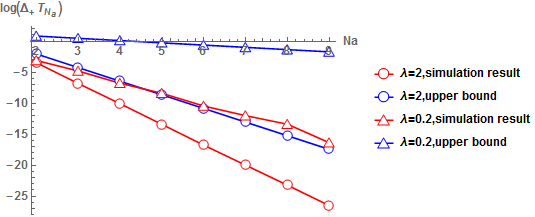
\includegraphics[width=250pt]{decreaing_exponential.png}
  \caption{连分式指数收敛性图示}\label{fig:continuous_fraction_exponential}
\end{figure}
根据图~\ref{fig:continuous_fraction_exponential}可以看出:
\begin{itemize}
\item 通过蒙特卡罗仿真进一步验证了定理~\ref{theorem:exponential_decreasing}的正确性。
\item $\lambda=\frac{a}{b}$,表示锚点定位强度与目标节点协作强度之比,当$\lambda$较大即锚点定位更强时,图中协作信息量下降得更快,表明更远的协作链路所能提供的信息更少。
\item 实际随机模拟中的信息衰减速度要快于定理~\ref{theorem:exponential_decreasing}给出的上界,这主要是因为随机模拟中出现角度正交的情况时会阻断信息量从较远链路的传播。为了讨论信息衰减下界,我们下面假设链路的夹角$\theta_i$服从零均值的正态分布,对于给定的$\Delta \theta$标准差$\sigma$满足$3\sigma=\Delta \theta$,由$3-\sigma$原则可近似认为角度变化不会超过$\Delta$.
\end{itemize}
\end{remark}
\begin{remark}
在\ref{subsection:temporal_cooperative_localization}小节中,推导得出两个节点时间一次协作的模型问题可以转化为单节点的模形,但存在一个区别在于这里各时刻速度方向$\theta_i$是随机变量,因此求得的SPEB$\frac{1}{\lambda}+\frac{1}{T_1}$是关于$\theta_i$的随机变量,要对其求数学期望才能得到平均性能。

沿用式\ref{eq:recursive_efim}的假设,对诸$\theta_i$求平均后即得平均性能,由于是连分式的形式无法显式给出平均后的结果,但在后续仿真中我们将分别采用蒙特卡罗模拟的方法估计这个平均性能。

另外由于定理~\ref{theorem:exponential_decreasing}中的信息衰减上下界不含$\theta$,因此也是平均性能提升的衰减速率。如果针对两个节点时间协作的模型问题,则应
估计$\sum_{i=N_a}^{2N_a}\frac{1}{q^{2i}}$,结果还是$q^{2N_a}$量级,即$N_a$层后面的所有链路的增益与第$N_a$层的增益相当,即我们有如下推论,详见附录[\ref{B_F_5}]:
\end{remark}
\begin{corollary}[定理\ref{theorem:exponential_decreasing}的推论]\label{corollary:exponential_decreasing}
在定理\ref{theorem:exponential_decreasing}的的条件下,数列$\{T_{N_a}\}$收敛于$T_{\infty}$,收敛速度是超线性收敛的,即\[
\exists q>1,s.t. \lim_{N_a\to\infty}\frac{T_{N_a}-T_{\infty}}{(T_{N_a+1}-T_{\infty})^q}>0
\]
\end{corollary}
上面的推导过程具有一般性,下面我们不对未知节点测距方差作出相等的假设,则对$a\bm{I}+b\bm{J}$提取a,并设$\lambda_{ij}=\frac{b}{a\sigma_{ij}^2}$于是我们只需考虑$\bm{I}+\bm{J}$,其中
\[\scriptsize{
J=\left(
\begin{array}{ccccc}
\lambda_{12}\bm{u}_{12}\bm{u}_{12}^T&-\lambda_{12}\bm{u}_{12}\bm{u}_{12}^T&\bm{0}&\dots&\bm{0}\\
&&&&\\
-\lambda_{12}\bm{u}_{12}\bm{u}_{12}^T&\lambda_{12}\bm{u}_{12}\bm{u}_{12}^T+&-\lambda_{23}\bm{u}_{23}\bm{u}_{23}^T&\dots&0\\
&\lambda_{23}\bm{u}_{23}\bm{u}_{23}^T&&&\\
\vdots &\vdots&\ddots &\vdots&\vdots\\
\bm{0}&\dots&\bm{0}&-\lambda_{N-1,N}\bm{u}_{N-1,N}\bm{u}_{N-1,N}^T&\lambda_{N-1,N}\bm{u}_{N-1,N}\bm{u}_{N-1,N}^T\\
\end{array}
\right)}
\]
类似式~(\ref{eq:recursive_efim}),
我们可以导出目标节点等效费舍尔信息矩阵一个特征值为1,另一个特征值$T_1$满足下面的递推关系式:
\begin{equation}\label{eq:recursive_efim_second}
  T_i=\frac{1}{\lambda_{i,i+1}^{-1}+\sin^2\theta_i+\frac{\cos^2\theta_i}{T_{i+1}}}
\end{equation}
其基本形式和(\ref{eq:recursive_efim})相同,计算算到$T_{N_a}=1$,
具体推导过程可参考[\ref{B_F_3}]

并且可以证明,减小诸$\theta$可以提高$T_1$即增大信息量,因此在线性网络中,当目标节点作直线运动时,确定其各个时刻的位置获得的信息量最大,因而精度最高。
\subsection{正方形网络与正六边形网络平均定位误差求解}\label{subsection:square_and_hexagon_network}
在协作定位网络的问题模型下,我们利用等效费舍尔信息矩阵的数学工具,考虑大规模空间协作两种特殊的情形:
正方形网络和正六边形网络。正六边形网络的每个内部节点周围有3个节点与之协作,且该内部节点位于周围三个节点构成的正三角形的重心上。
为研究正六边形网络对定位性能的影响,我们考虑以一个节点$\bm{p}$为网络中心,我们称网络中某节点$\bm{p}_n$位于第n层链路上如果$\bm{p}_n$到$\bm{p}$的最短路径为n,图\ref{HexagonNetwork}就是一个只考虑前两层链路的正六边形网络。
\begin{figure}[h]
  \centering
  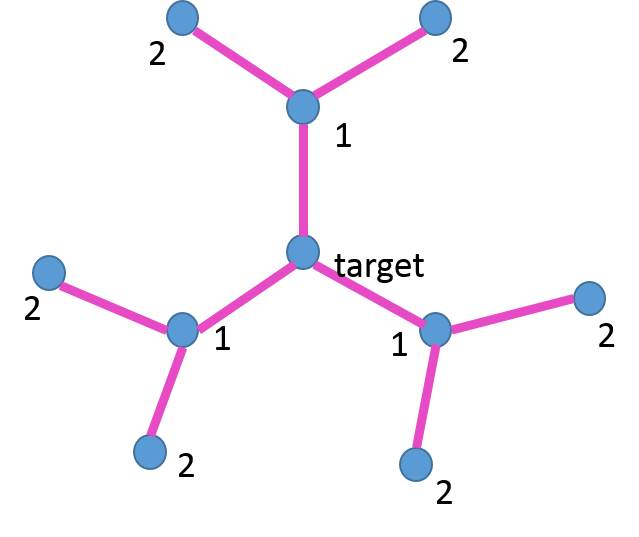
\includegraphics[width=250pt]{massive_spatial.png}
  \caption{只考虑前两层链路的正六边形网络}\label{HexagonNetwork}
\end{figure}

正方形网络的描述同正六边形网络,如果以目标节点作为坐标原点,含其他未知位置的节点的两条直线作为坐标轴建立平面直角坐标系,
根据前面的正交性的结论,非坐标轴上的点不会对目标节点提供定位信息,而两条坐标轴提供的信息又彼此独立,因此其定位信息量是2个完全相同的部分相加,
每部分由式(\ref{eq:gcf_1})描述,在网络规模很大时近似于极限值$\sqrt{\lambda^2+4\lambda}$。

该结论可以推广至一般矩形网络,且各节点相互测距的方差$\sigma^2_{i,j}$不相等,由式(\ref{eq:recursive_efim_second})可以看出正交性的结论仍然成立,因此非坐标轴上的点不会对目标节点提供定位信息,在实际定位系统的设计中,非坐标轴上的点的信息无需传到目标节点或中央处理器进行解算。

下面我们给出大规模正六边形网络目标节点定位误差界的解析表达式,首先需要下面的引理,推导过程见附录[\ref{B_F_4}]
\begin{lemma}\label{lemma:hexagon}
  设$u$是模长为1的平面向量,那么有:
\begin{equation}\label{eq:equiv}
  u^T((\lambda+\frac{3}{2})I_2-\frac{1}{\lambda+\frac{3}{2}}(\frac{3}{2}I_2-uu^T))^{-1}u
  =((\lambda+\frac{3}{2})-\frac{1/2}{\lambda+\frac{3}{2}})^{-1}
\end{equation}
\end{lemma}
  上面的引理能够把连分式中与$u$相关的项化为与$u$无关的项,由此推出度为3的协作网络中心节点SPEB为:
  \[
\lambda+\frac{3}{2}-\cfrac{3/2}{\lambda+\frac{3}{2}-\cfrac{1/2}{\lambda+3/2-\dots}}
  \]
  注意到除了第一层的协作外,后面每层协作由于前一层的削弱系数由3/2变为1/2.
  用同样的方法可求出极限值为:
  \[
  \sqrt{\lambda^2+3\lambda+\frac{1}{4}}-\frac{1}{\lambda+\frac{3}{2}+\sqrt{\lambda^2+3\lambda+\frac{1}{4}}}
  \]
  取倒数即为某方向的误差下界,由于网络的各向同性,x方向和y方向的误差下界都是这个数。
该误差下界总是比正方形网格x或y方向的误差大。

\section{结论}\label{section:conclusion}
  % Keep the summary *very short*.
  \begin{itemize}
  \item
  数学方法方面
  \begin{itemize}
  \item 本文的推导首先要处理对称正定的矩阵,因此本文会应用已有的结果如求一个矩阵的逆阵的某个子式的公式、关于矩阵逆的恒等式等结论来对要研究的矩阵进行预处理
  \item 其次由于很多时候直接推导存在很大的困难,需要先归纳后证明,本文充分利用了数学归纳法完成这一任务
  \item 最后推导得出的表达式往往比较复杂,表达式的化简需要特殊的数学方法,本文根据问题的特征分别采用了瑞利商、黎曼积分以及连分式等思路
  \end{itemize}
  \item
    已取得的成果
  \begin{itemize}
  \item
    使用复数表示法推导得出非协作定位场景下费舍尔信息矩阵的特征值和特征向量的表达式.
  \item
    推导得出秩一矩阵的克罗内克积对N维对称正定矩阵扰动后行列式的表达式
  \item
    推导得出二维场景下特殊完全图的邻接矩阵所有特征值,其中使用瑞利商给出了最大 特征值的表达式
  \item 推导得出二维场景下特殊度为2的图的邻接矩阵的所有特征值;当网络规模趋向无穷大时,求出了所有特征值的倒数和的平均值的极限
  \item 使用连分式推导得出对称正定矩阵$\bm{A}$确定的$\bm{A}^{-1}_{1\times2,1\times2}$的两个特征值;分析得出了决定特征值的连分式的序列指数收敛的特性。
  \end{itemize}
  \end{itemize}
